\setcounter{section}{3}
\setcounter{subsection}{1}
\subsection{実行環境モデル}
プロシージャについて考え始めた時に, 置換モデルを導入した.
そのモデルでは, プロシージャを適用するために, プロシージャの中身での
仮引数の出現をその引数の値に変えることで実行することができる.
もう一度例を挙げると

\begin{lstlisting}[basicstyle=\footnotesize]
(define (square x) (* x x))
\end{lstlisting}
\noindent
という定義で

\begin{lstlisting}[basicstyle=\footnotesize]
(square 2)
\end{lstlisting}
\noindent
を実行しようと思えば, \lstinline{square}の中の\lstinline{x}を
\lstinline{2}に変えれば良い. なので, \lstinline{(* 2 2)}
を実行することになる.

しかしながら, 代入の概念が入ってしまうと, 以上のモデルが成り立たなくなる.
例えば,

\begin{lstlisting}[basicstyle=\footnotesize]
(define (foo x)
  (set! x 1)
  (+ x 1))
\end{lstlisting}

のようなプロシージャについて考えると, \lstinline{(foo 5)}で呼びだした時に,
置換モデルを用いると, \lstinline{x}が\lstinline{5}に置換されて,
\lstinline{(set! 5 1)}が実行できたとしても, \lstinline{6}という誤った結果に
なってしまう.

問題点としては, 変数は単なる値ではなく, 値が保存されている場所を指していると
考えられる. 新しい実行モデルでは, 値が保存される場所は「環境」という構造を持って
表す.

環境はフレームのシーケンスであり, フレームはバインディングのテープルである.
ここでは, バインディングは変数名とその値を結ぶものである.
フレームはグローバルのもの以外は自分の実行環境のポインタを持つ. 変数の値は
一番最初のフレームでのバインディングで決まる. どのフレームにもバインディングが
なければ, 値がバインドされていないという.

\begin{figure}[ht]
  \centering
  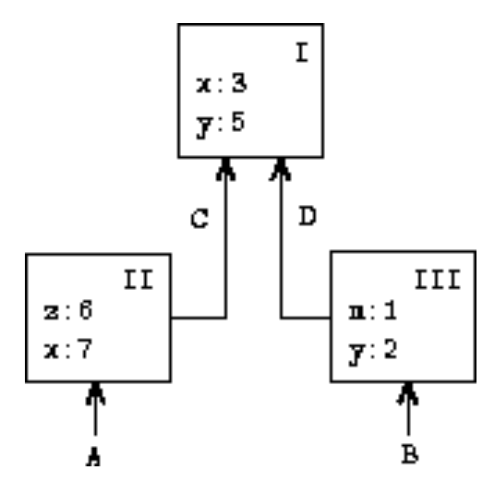
\includegraphics[height=5cm,width=5cm]{imgs/environment_example.png}
  \caption{\label{fig:env-example}実行環境の構造}
\end{figure}

例えば, 図\ref{fig:env-example}では, フレームは3つ存在する.
グローバル環境で\lstinline{x}の値としてフレーム\lstinline{I}
が採用されるので\lstinline{3}になるが, \lstinline{A}環境で実行すると,
フレーム\lstinline{II}の値が採用され, \lstinline{x}の値が\lstinline{7}になる.
同じく, \lstinline{y}をグローバル環境で実行すると値が\lstinline{5}になるが,
\lstinline{B}環境で実行すると, 値が\lstinline{2}になる.

実行する時に, 環境によって式がどう評価されるのかが決まるので, 式そのものだけでは
意味を持つではなく, ある環境で式が意味を持つと言える.
%
\subsubsection{評価ルール}
全体的な評価ルールは置換モデルの時と変わらない.

\begin{itemize}
\item 複合式の部分式を評価する
\item オペレーターをオペランドの部分式の値に適用する
\end{itemize}

しかし, 環境モデルではプロシージャを適用する時, 評価ルールが変わってくる.
環境モデルにおいて, プロシージャはコードと環境へのポインタの組み合わせで定義される.
プロシージャを作る唯一の方法は, \lstinline{lambda}式を評価することである.
例えば,

\begin{lstlisting}[basicstyle=\footnotesize]
(define (square x) (* x x))
\end{lstlisting}
が
\begin{lstlisting}[basicstyle=\footnotesize,caption=]
(define square (lambda (x) (* x x)))
\end{lstlisting}
として評価されるので, グローバル環境で\lstinline{square}に
\lstinline{lambda}式をバインドする.

\begin{figure}[h]
  \centering
  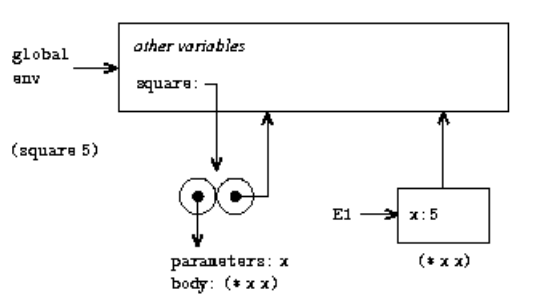
\includegraphics[height=5cm,width=12cm]{imgs/square_env.png}
  \caption{\label{fig:square-env}グローバル環境での\lstinline{(square 5)}の実行}
\end{figure}


環境モデルでは, プロシージャの適用は以下の2つのルールでまとめることができる.
\begin{itemize}
\item プロシージャは\lstinline{lambda}式を評価することによって作成される.
  プロシージャは環境を持つので, コードと環境へのポインタの組み合わせとして定義される.
\item プロシージャの適用の時, 新しいフレームが作成される.
  そのフレームの環境はプロシージャの環境となる.
  新しく作られたフレームで仮引数が実引数にバインドされる.
\end{itemize}

図\ref{fig:square-env}で実行例を示す.